\ifx\wholebook\relax \else

\documentclass[b5paper]{ctexart}
\usepackage[nomarginpar
  %, margin=.5in
]{geometry}

\addtolength{\oddsidemargin}{-0.05in}
\addtolength{\evensidemargin}{-0.05in}
\addtolength{\textwidth}{0.1in}

\usepackage[cn]{../prelude}

\setcounter{page}{1}

\begin{document}

\title{数的诞生}

\author{刘新宇
\thanks{{\bfseries 刘新宇} \newline
  Email: liuxinyu99@hotmail.com \newline}
  }

\maketitle
\fi

\markboth{数的诞生}{数的旅程}

\ifx\wholebook\relax
\chapter{数的诞生}
\numberwithin{Exercise}{chapter}
\fi

\epigraph{一二三四五,金木水火土。天地分上下,日月照今古。}{——部编小学一年级语文课本第一课}

数充满了我们的生活。早上6:30起床,日历上是2025年2月17日。手机电量已经充到99\%。有同学在社交网络的班级群里说:“2025年是神奇的一年,2025是45的平方。”我点了“+1”,现在这条消息有36个\heartsuit{}了。我喝了200毫升牛奶,吃掉了3个包子,花了15分钟骑自行车到学校。今天的8节课中有2节是数学……

这短短的150字中有14个数字。数是谁发明的?历史书上没有答案。数出现在所有历史文字记录中,数也许诞生在史前,伴随着语言和文字。要找到答案,我们有两条线索:1、追寻古老的历史物证,石刻、壁画、器物上关于数的印记;2、追溯数在语言演变中的痕迹。比如英文中的eleven (11)来自古英语endleofan,意思是(数到10还)剩余1;tweleve (12)来自twelf,意思是剩余2。

\section{数的诞生}

\begin{figure}[htbp]
 \centering
 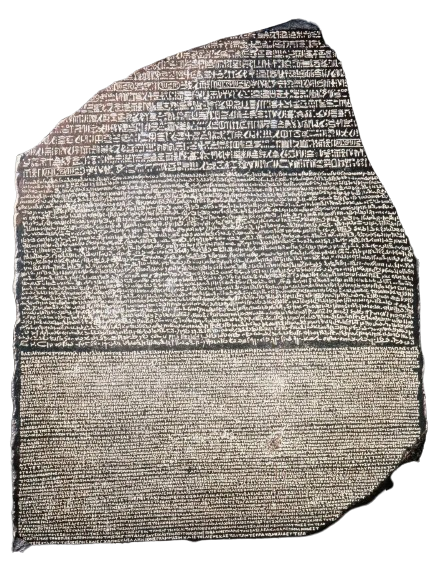
\includegraphics[scale=0.4]{img/rosetta-stone}
 \caption{罗赛塔石碑,古埃及,公元前196年}
 \label{fig:rosetta-stone}
\end{figure}


\ifx\wholebook\relax \else
\section{参考答案}
\shipoutAnswer

\begin{thebibliography}{99}

%% \bibitem{wiki-number}
%% Wikipedia. ``古代计数系统的历史''. \url{https://en.wikipedia.org/wiki/History_of_ancient_numeral_systems}

%% \bibitem{trip-to-number-kingdom}
%% [美]\ 卡尔文$\cdot$C$\cdot$克劳森\ 著\ 袁向东、袁钧\ 译. ``数学旅行家:漫游数王国''. 上海教育出版社。ISBN: 7-5320-7883-3/G $\cdot$ 7972

%% \bibitem{wiki-babylonian-num}
%% Wikipedia. ``古巴比伦数字''. \url{https://en.wikipedia.org/wiki/Babylonian_numerals}

\end{thebibliography}

\expandafter\enddocument
%\end{document}

\fi
